\subsection{Digitale filtre}
% IIR 
% FIR
% Moving average
% threathold 


Et filter har typisk til formål at frafiltrere uønskede frekvenser fra signalet\fxnote{opg: andre formål}. Ønskes det at fjerne høje frekvenser, anvendes et lavpasfilter, som lader frekvenser under en valgt værdi passere, mens der, hvis man ønsker de lave frekvenser fjernet, anvendes et højpasfilter, som lader de høje frekvenser over en valgt værdi passere. Disse to filtertyper kan kombineres alt efter om man vil fjerne frekvenser udenfor et bestemt spektrum, båndpasfilter, eller kun vil fjerne en lille del af spektret, båndstopfilter, hvilket er illustreret på \figref{fig:filtre}\fxnote{opg: skal figuren være der?}. Ved en sammensætning hvor lavpasfilteret dæmper efter højpasfilteret, og højpasfilteret dæmper før lavpasfilteret, fås et båndpasfilter. Sammensættes de to filtre modsat med et lavpasfilter som dæmper før højpasfilteret mens højpasfilteret efter lavpasfilteret, fås et båndstopfilter.\fxnote{opg: Overvej om dette skal være her.}
\citep{Ramsden2001}

\begin{figure}[H]
	\centering
	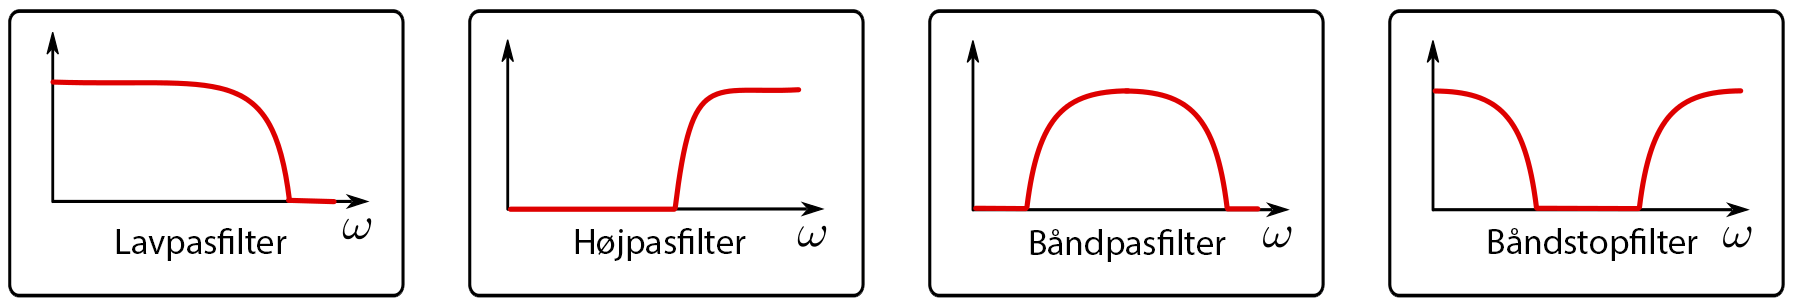
\includegraphics[scale=0.2]{figures/bProblemloesning/filtre.png}
	\caption{På figuren ses ... \citep{Aasvik2016} (Modificeret)}
	\label{fig:filtre}
\end{figure}

FILTERTYPER

Infinite impulse response (IIR)
- Butterworth
- chebyshev 
- ect. 
Finite impulse response (FIR)
- Parks-McClellan algorithm
- Frequency sampling
- window type
- ??




\subsubsection{Filterdesign}


Design af filtre: 
- start med hvilket frekvensspectrum signalet har.
- herved finder man også ud af om det skal være lavpas, højpas, båndstop eller båndpas filter
- samplerate
- ripples


the result of the design process is typically a transfer function in z. 

(test af filter : Inden det implementeres testes det som virker mest oplagt, men også andre muligheder —> den løsning som kommer tættest på specifikationerne, vælger man —> efter implementeringen testes det igen, om det opfører sig)


The analysis of digital filters centers on the transfer function. The transfer function is taken as the description of the filter prior to implementation. If we have the transfer function description, we can determine mathematically what we can expect out of the filter upon implementation, in the best case. From the transfer function, we can determine the impulse response, the stability of the filter, the steady-state frequency respons, the difference equation, and the response to an arbitrary input.

\citep{Blandford2013}



\subsubsection{FIR filtre}
FIR filtre er defineret som digitale filtre med endeligt mange impuls responser.

\begin{flalign}
	Y[n] = \sum_{m=0}^{m} b_m X[n-m]
	\label{eq:fir}
\end{flalign}

Denne filtertype kan designes med en lineær fase, mens IIR filtre kun tilnærmelsesvis kan designes lineære.
--> dette er grunden til at FIR i nogle tilfælde foretrækkes.
Når der designes et FIR filter med lineær fase, benyttes ofte Fourier serier

Der findes to typer af FIR filtre for symmetrisk impuls respons; type 1 som har lige orden, men ulige længde, og type 2 som har en ulige orden, men en lige længde. Disse kan skrives som en sum af cosinus funktioner.
Der findes ligeledes to typer af FIR filtre for asymmetrisk impuls respons; type 3 som har lige orden, men ulige længde, og type 2 som har en ulige orden, men en lige længde. Disse kan skrives som en sum af sinus funktioner.
De forskellige typer egner sig hver i sær bedst til forskellige filtre, som det ses i \tabref{tab:FIR_typer}. \citep{Blandford2013}

\begin{table}[H]
	\centering
	\caption{Tabellen illustrerer hvilke FIR typer som egner sig bedst til forskellige filtre. \citep{Blandford2013} (modeficeret)}
	\begin{tabular}{cccc}
		Type & Symmetri                                                           & Forbehold                                                       & Egner sig til                                                                \\
		1    & \begin{tabular}[c]{@{}c@{}}Ulige længde\\ Symmetrisk\end{tabular}  & Ingen                                                           & \begin{tabular}[c]{@{}c@{}}Lavpas\\ Højpas\\ Båndpas\\ Båndstop\end{tabular} \\
		2    & \begin{tabular}[c]{@{}c@{}}Lige længde\\ Symmetrisk\end{tabular}   & $H(f_s/2)=0$                                                    & \begin{tabular}[c]{@{}c@{}}Lavpas\\ Højpas\end{tabular}                      \\
		3    & \begin{tabular}[c]{@{}c@{}}Ulige længde\\ Asymmetrisk\end{tabular} & \begin{tabular}[c]{@{}c@{}}$H(0)=0$\\ $H(f_s/2)=0$\end{tabular} & \begin{tabular}[c]{@{}c@{}}Højpas\\ Differentiator\end{tabular}              \\
		4    & \begin{tabular}[c]{@{}c@{}}Lige længde\\ Asymmetrisk\end{tabular}  & $H(0)=0$                                                        & \begin{tabular}[c]{@{}c@{}}Højpas\\ Differentiator\end{tabular}             
	\end{tabular}
	\label{tab:FIR_typer}
\end{table}

FIR filtre optræder som forskellige konstruktioner, blandt andet Parks-McClellan algoritmen, Frekvens sampling og window type \fxnote{opg: hvilke andre?}.

Parks-McClellan algoritmen:





Frekvens sampling: 






Windowing:
Når der benyttes Fourier serier til at lave et ideelt FIR filter, fås en række koefficienter mellem minus uendelig og plus uendelig. Da et uendelig langt filter ikke kan implementeres, forkortes antallet af koefficienter til et antal som kan implementeres og stadig tilnærmelsesvis giver et ideelt filter. Matematisk sker dette ved at gange impulsresponsen med et rektangulært window. 

Diskret fourier transformation (DFT) af et rektangulært window i tidsdomænet, giver en sinusfunktion i frekvensdomænet.

\begin{flalign}
Y[n] = H*W = \sum_{k=0}^{\infty} H[k] \cdot W[n-k]
\label{eq:window}
\end{flalign}





Derudover kan filtrene implementeres på forskellig vis, alt efter deres formål. Moving average benyttes til at udglatte signalet, ved at finde gennemsnitsværdien for et bestemt antal samples:

\begin{flalign}
	avg = \frac{1}{N} \sum_{i=1}^{N} x_i
	\label{eq:mavg}
\end{flalign}








\subsubsection{IIR filtre}
IIR filtre er defineret som digitale filtre med uendeligt mange impuls responser. 

\begin{flalign}
	Y[n] = \sum_{k=1}^{k} a_k Y[n-k] + \sum_{m=0}^{m} b_m X[n-m]
	\label{eq:iir}
\end{flalign}




Infinite impulse response (IIR)
- Butterworth
- chebyshev 
- ect. 


